\documentclass[en,hazy,blue,screen,14pt]{elegantnote}

\title{PostgreSQL Core Technology Training}

\author{Xiao Bu}
\institute{https://cherry-creek.net}

% \version{2.50}
% \date{Dec. 31, 2022}

\begin{document}
\maketitle
% logo
\centerline{\includegraphics[width=0.5\textwidth]{ccalogo.pdf}}


% =========================================
\newpage
\section{Install PostgreSQL From Source Code}
\centerline{\includegraphics[width=0.8\textwidth]{client_server.pdf}}

% A debugger is a program that simulates/runs another program and allows you to do the following things: 
% \begin{itemize}
%   \item Pause and continue its execution.
% \end{itemize}

% =========================================
\newpage
\section{Some Fundamental Concepts}
\begin{itemize}
	\item Bit and Byte
	\item Files and Memory
	\item Program and Process
	\item Private Memory and Shared Memory
\end{itemize}

\centerline{\includegraphics[width=0.5\textwidth]{computer.pdf}}

% =========================================
\newpage
\section{Computer Overview}
\centerline{\includegraphics[width=1.0\textwidth]{hardware_software.pdf}}

% =========================================
\newpage
\section{Bit and Byte}
\begin{itemize}
	\item Bit: binary digit, is the most basic unit of information. It represents a logical state with one of two possible values such as "0" and "1".
	\item Byte: a byte is a sequence of 8 bits.
\end{itemize}
\centerline{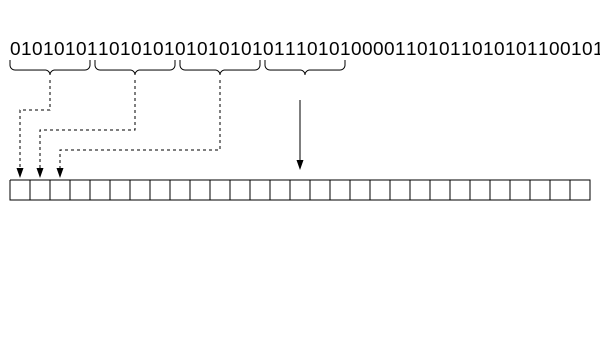
\includegraphics[width=0.8\textwidth]{memory1.pdf}}

% =========================================
\newpage
\section{The Value Range of a Byte}
\begin{itemize}
	\item The minimum value of a byte is 0.
	\item The maximum value of a byte is 255.
\end{itemize}
\centerline{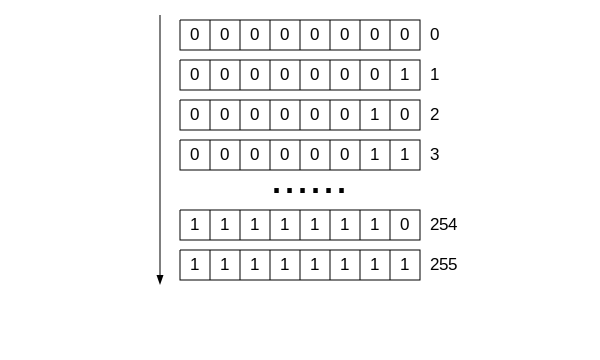
\includegraphics[width=0.8\textwidth]{byte_range.pdf}}

% =========================================
\newpage
\section{What is File?}
\begin{itemize}
	\item A computer file is a collection of data on a computer storage device, primarily identified by its filename.
	\item Files are organized into one-dimensional arrays of bytes. Any file is a sequence of bytes, nothing more and nothing less.
\end{itemize}
\centerline{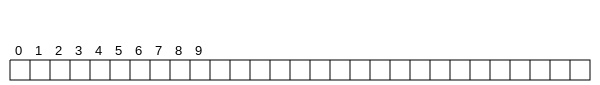
\includegraphics[width=1.0\textwidth]{memory_model.pdf}}

% =========================================
\newpage
\section{What is Offset?}
\begin{itemize}
	\item Offset within an array is an integer indicating the distance between the beginning of the object and a given element.
	\item The concept of a distance is valid only if all elements of the object are of the same size (typically given in bytes or words).
\end{itemize}
\centerline{\includegraphics[width=1.0\textwidth]{file_offset.pdf}}

% =========================================
\newpage
\section{Overview of Shared Memory in Postgres}
\begin{itemize}
	\item Offset within an array is an integer indicating the distance between the beginning of the object and a given element.
\end{itemize}
\centerline{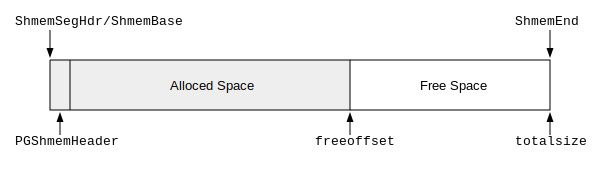
\includegraphics[width=1.0\textwidth]{shared_memory_overview.pdf}}

% =========================================
\newpage
\section{What is Program?}
\begin{itemize}
	\item A computer program is a sequence of instructions in a programming language for a computer to execute.
	\item A computer program in its human-readable form is called source code. 
	\item Source code may be translated to machine instructions using a compiler written for the language. The resulting file is called an executable.
\end{itemize}

\centerline{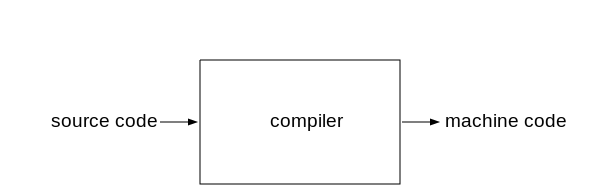
\includegraphics[width=1.0\textwidth]{source_compile.pdf}}

% =========================================
\newpage
\section{What is Process?}
\begin{itemize}
	\item X.
\end{itemize}
\centerline{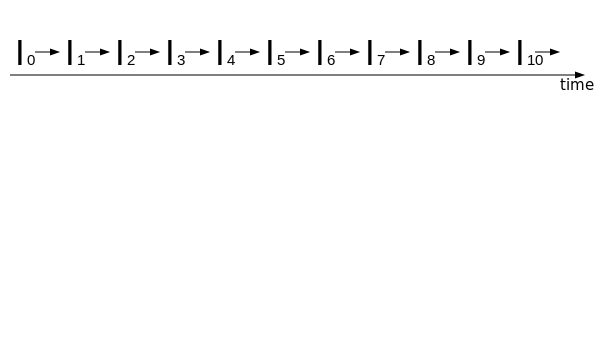
\includegraphics[width=1.0\textwidth]{process.pdf}}

% =========================================
\newpage
\section{The Memory of a Process}
\begin{itemize}
	\item X.
\end{itemize}
\centerline{\includegraphics[width=1.0\textwidth]{process_memory.pdf}}


% =========================================
\newpage
\section{How to Create a New Process?}
\begin{itemize}
	\item X.
\end{itemize}
\centerline{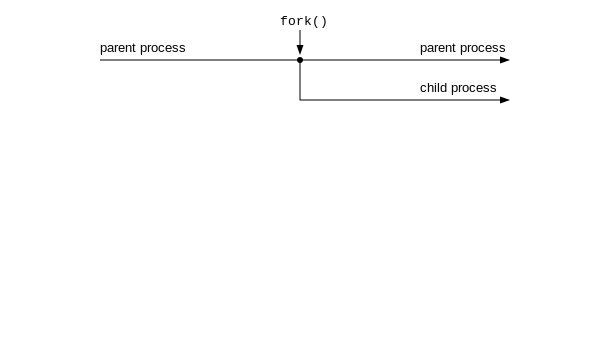
\includegraphics[width=1.0\textwidth]{fork_process.pdf}}


% =========================================
\newpage
\section{What is X?}
\begin{itemize}
	\item X.
\end{itemize}
\centerline{\includegraphics[width=1.0\textwidth]{file_offset.pdf}}

% =========================================
\newpage
\section{What is X?}
\begin{itemize}
	\item X.
\end{itemize}
\centerline{\includegraphics[width=1.0\textwidth]{file_offset.pdf}}

% =========================================
\newpage
\subsection{Optional Modes}

This template provides optional modes: good for eye mode (geye) and hazy mode, while the paper color is green for the former and light blue for the latter. you can use the following code to activate the desired mode:
\begin{lstlisting}[frame=none]  
  \documentclass[geye]{elegantnote} % or
  \documentclass[mode=geye]{elegantnote}
  \documentclass[hazy]{elegantnote} % or
  \documentclass[mode=hazy]{elegantnote}
\end{lstlisting}

\begin{remark}
  If you are expected to customize background, use:
  \begin{lstlisting}
    \definecolor{geyecolor}{RGB}{199,237,204}
    \pagecolor{geyecolor}
  \end{lstlisting}
\end{remark}

\newpage
\subsection{Device Options}

To make the notes more comfortable to read, we designed four output options (of different sizes) that correspond to different reading devices: Pad (default), Kindle, PC and A4paper. 

\textcolor{red}{New}: For the convenience of notes presentation, version 2.20 offers a new option for device, i.e. \lstinline{device=screen}, which is similar to the size of MS Powerpoint with ratio aspect of 4:3 (2019/12/06).

The options of output for different devices are
\begin{lstlisting}[frame=none]  
  \documentclass[device=pad]{elegantnote}    % ipad screen size
  \documentclass[device=kindle]{elegantnote} % kindle screen size
  \documentclass[device=pc]{elegantnote}     % double pages for pc 
  \documentclass[device=normal]{elegantnote} % a4 normal page
  \documentclass[device=screen]{elegantnote} % 4:3 PPT size
\end{lstlisting}

\begin{note}
You can also select the device by using a direct assignment method, such as:
\end{note}

\begin{lstlisting}[frame=none]  
  \documentclass[pad]{elegantnote}
  \documentclass[kindle]{elegantnote}
  \documentclass[pc]{elegantnote}
  \documentclass[normal]{elegantnote}
  \documentclass[screen]{elegantnote}
\end{lstlisting}

\begin{note}
To get a normal A4paper size PDF, please select \lstinline{device=normal}.
\end{note}

\subsection{Math Fonts}

This template defines a new option (\lstinline{math}), with three options:

\begin{enumerate}
  \item \lstinline{math=cm} (default), use \LaTeX{} default math font (recommended).
  \item \lstinline{math=newtx}, use \lstinline{newtxmath} math font (may bring about bugs).
  \item \lstinline{math=mtpro2}, use \lstinline{mtpro2} package to set math font.
\end{enumerate}

\newpage
\subsection[Color Themes]{Color Themes\footnote{Test for chapter footnote.}}

This template contains 5 color themes, \textcolor{egreen}{green}, \textcolor{ecyan}{cyan}, \textcolor{eblue}{blue}(default), \textcolor{sakura}{sakura} and \textcolor{black}{black}. If you don't need color, you can choose black theme. The color theme is enabled in the same way as before:
\begin{lstlisting}[frame=none]  
  \documentclass[green]{elegantnote}
  \documentclass[color=green]{elegantnote}
  ....
  \documentclass[black]{elegantnote}
  \documentclass[color=black]{elegantnote}
\end{lstlisting}


\subsection{Languages}

This template contains two sets of language environments, changing the language environment will change the title of table/figure (figure, table), article structure words (such as the table of contents, references, etc.), and the environment Introductory words (such as Theorem, Lemma, etc.). The different language modes are enabled as follows:
\begin{lstlisting}[frame=none]  
  \documentclass[cn]{elegantnote}
  \documentclass[lang=cn]{elegantnote}
  \documentclass[en]{elegantnote}
  \documentclass[lang=en]{elegantnote}
\end{lstlisting}

\begin{note}
Chinese characters are allowed in Chinese mode only. To type in Chinese characters in English mode, please include \lstinline{ctex}\footnote{Please use \lstinline{scheme=plain} to retain headlines in English.} or \lstinline{xeCJK} package.
\end{note}


\subsection{Theorem Class Environments}

This template used the \lstinline{amsthm} to create theorems, there are 4 types of theorem environments
\begin{itemize}
  \item \textbf{Theorem-Class}: theorem, lemma, proposition, corollary;
  \item \textbf{Definition-Class}: definition, conjecture, example;
  \item \textbf{Remark-Class}: remark, note, case;
  \item \textbf{Proof-Class}: proof.
\end{itemize}

\begin{remark}
With the option \lstinline{lang=cn} , the introductory words of the theorem class environments will be changed to Chinese.
\end{remark}


\section{Writing Sample}

We will define the integral of a measurable function in three steps. First, we define the integral of a nonnegative simple function. Let $E$ be the measurable set in $\mathcal{R}^N$.

% source: https://www.maths.tcd.ie/~dwilkins/LaTeXPrimer/Theorems.html

\begin{definition}[Left Coset]
Let $H$ be a subgroup of a group~$G$.  A \emph{left coset} of $H$ in $G$ is a subset of $G$ that is of the form $xH$, where $x \in G$ and $xH = \{ xh : h \in H \}$. Similarly a \emph{right coset} of $H$ in $G$ is a subset of $G$ that is of the form $Hx$, where $Hx = \{ hx : h \in H \}$
\end{definition}

Note that a subgroup~$H$ of a group $G$ is itself a left coset of $H$ in $G$.

\begin{lemma}[Size Of Left Coset]
Let $H$ be a finite subgroup of a group $G$.  Then each left
coset of $H$ in $G$ has the same number of elements as $H$.
\end{lemma}

\begin{theorem}[Lagrange's Theorem]
Let $G$ be a finite group, and let $H$ be a subgroup
of $G$.  Then the order of $H$ divides the order of $G$.
\end{theorem}

\begin{proof}
Let $z$ be some element of $xH \cap yH$.  Then $z = xa$ for some $a \in H$, and $z = yb$ for some $b \in H$. If $h$ is any element of $H$ then $ah \in H$ and $a^{-1}h \in H$, since $H$ is a subgroup of $G$. But $zh = x(ah)$ and $xh = z(a^{-1}h)$ for all $h \in H$. Therefore $zH \subset xH$ and $xH \subset zH$, and thus $xH = zH$.  Similarly $yH = zH$, and thus $xH = yH$, as required.
\end{proof}

\begin{figure}[!htbp]
	\centering
	\includegraphics[width=0.6\textwidth]{scatter.pdf}
	\caption{Matplotlib: Scatter Plot Example\label{fig:mpg}}
\end{figure}

Regression analysis is a powerful statistical method that allows you to examine the relationship between two or more variables of interest. While there are many types of regression analysis, at their core they all examine the influence of one or more independent variables on a dependent variable. The process of performing a regression allows you to confidently determine which factors matter most, which factors can be ignored, and how these factors influence each other.

Let's continue using our application training example. In this case, we'd want to measure the historical levels of satisfaction with the events from the past three years or so, as well as any information possible in regards to the independent variables. 

\begin{table}[htbp]
  \small
  \centering
  \caption{Auto MPG and Price \label{tab:reg}}
    \begin{tabular}{lcc}
    \toprule
                    &       (1)         &        (2)      \\
    \midrule
    mpg             &    -238.90***     &      -49.51     \\
                    &     (53.08)       &      (86.16)    \\
    weight          &                   &      1.75***    \\
                    &                   &      (0.641)    \\
    constant        &     11,253***     &       1,946     \\
                    &     (1,171)       &      (3,597)   \\
    obs             &        74         &         74     \\
    $R^2$           &      0.220        &       0.293    \\
    \bottomrule
    \multicolumn{3}{l}{\scriptsize Standard errors in parentheses} \\
    \multicolumn{3}{l}{\scriptsize *** $p<0.01$, ** $p<0.05$, * $p<0.1$} \\
    \end{tabular}%
\end{table}%


\begin{itemize}[noitemsep]
  \item Routing and resource discovery;
    \begin{itemize} 
      \item Language Models
      \item Vector Space Models
    \end{itemize}
  \item Resilient and scalable computer networks;
  \item Distributed storage and search.
\end{itemize}


\section{Acknowledgement}

Thank \href{https://github.com/sikouhjw}{sikouhjw} and \href{https://github.com/syvshc}{syvshc} for their quick response to Github issues and continuously support work for Elegant\LaTeX{}. Thank China\TeX{} and \href{http://www.latexstudio.net/}{LaTeX Studio} for their promotion. 


\section{FAQ}

\begin{enumerate}[label=\arabic*).]
	\item \textit{How to remove the information of version?}\\
    Please comment \lstinline|\version{x.xx}|.
	\item \textit{How to remove the information of date?}\\
	  Please type in \lstinline|\date{}|.
	\item \textit{How to add several authors?}\\
	  Use \lstinline{\and} in \lstinline{\author} and use \lstinline{\\} to start a new line.
    \begin{lstlisting}
      \author{author 1\\ org. 1 \and author 2 \\ org. 2 }
    \end{lstlisting}
\end{enumerate}


%\printbibliography[heading=bibintoc, title=\ebibname]

\end{document}
